%---------------------------------------------------------------
\subsection{Simplicial complexes and Stanley-Reisner rings}
\label{subsec: simplicial complexes and Stanley-Reisner rings}
%---------------------------------------------------------------
This section will outline the theory of simplicial complexes and Stanley-Reisner theory.
\begin{definition}
    A (finite, regular) \emph{simplicial complex} $\Delta$ on a vertex set $V = [n] :=\{1,\ldots,n\}$ is a collection of subsets $F\subseteq V$ called \emph{faces} such that if $F$ is a face of $\Delta$ and $G\subseteq F,$ then $G\in\Delta.$ The \emph{dimension} of a face $F$ is $\dim F = |F| - 1.$
\end{definition}
\begin{remark}
    We note that traditionally the definition of simplicial complexes also includes the stipulation that $\Delta$ is supported on $V$, meaning that every singleton $\{v\}$ for $v\in V$ is a face of $\Delta.$ 
    If $v\in V,$ but $\{v\}$ is not a face of $\Delta,$ then there exists no face of $\Delta$ containing $\{v\}.$ Thus, $\Delta$ is simply a simplicial complex on the vertex set $V\setminus\{v\}.$ Algebraically, this corresponds to including the variable $x_v$ in the Stanley-Reisner ideal of $\Delta$ (Definition~\ref{def: SR ideal}). 
    In this article, we allow singletons to be nonfaces in our definition of a simplicial complex. 
\end{remark}
We now give a series of short definitions required for working with simplicial complexes. For further background on simplicial complexes and Stanley-Reisner theory, we refer the reader to \cite{BrunsHerzog1993, MillerSturmfels2005,Stanley1996}. A \emph{nonface} is a subset $G\subseteq V$ such that $G$ is not a face in $\Delta$ and it is a \emph{minimal nonface} if there does not exist a nonface $H\subsetneq G$.  
A \emph{facet}, or \emph{maximal face}, is a face in $\Delta$ that is not properly contained in any other face of $\Delta$. The \emph{dimension} of a face $F$ is $\dim F = |F|-1$, and
\[
\dim\Delta = \max\{\dim F : F\text{ is a facet of }\Delta\}.
\]
If all facets of $\Delta$ have the same dimension, then $\Delta$ is called \emph{pure}.

If every subset of $V$ is a face of $\Delta,$ equivalently $\Delta$ has no nonfaces (other than vertex nonfaces), then $\Delta$ is called a \emph{simplex}. In this case, $V$ is the unique maximal facet of $\Delta$ and $\dim\Delta = |V|-1.$
A collection of faces $\Delta'\subseteq\Delta$ that is closed under subsets is also a simplicial complex and is called a \emph{subcomplex} of $\Delta.$ Given any face $F$ of a simplicial complex $\Delta,$ the collection $\overline{F} = \{G:G\subseteq F\}$ of all subsets of $F$ is closed under subsets, so $\overline{F}$ is also a subcomplex of $\Delta.$ In particular, it is the simplex on the vertices of $F.$ 
Two other important subcomplexes are the deletion of a vertex and link of a face.
\begin{definition}
\label{def: deletion and link of a simplicial complex}
Given a simplicial complex $\Delta$ on a vertex set $V$ and for any $v\in V$ the \emph{deletion of $v$} is 
\[
\del_v(\Delta) = \{F\in\Delta: v\not\in F\}
\]
and the \emph{link of a face $F\in\Delta$} is
\[
\lk_F(\Delta) = \{G\in\Delta : G\cap F = \varnothing \text{ and }G\cup F\in\Delta\}.
\]    
When $F = \{v\}$ is a singleton we write $\lk_v(\Delta)$ for $\lk_{\{v\}}(\Delta).$
\end{definition}
\begin{definition}[\cite{bjorner1996shellable,provan1980decompositions}]
\label{def: vertex-decomposable}
    A (finite, regular) simplicial complex $\Delta$ on $n$ vertices is \emph{vertex decomposable} if
    \begin{itemize}
        \item $\Delta$ is a simplex; or
        \item there exists a vertex $v\in V$ such that
        \begin{enumerate}
            \item $\del_v(\Delta)$ is vertex decomposable,
            \item $\lk_v(\Delta)$ is vertex decomposable, and 
            \item $v$ is a \emph{shedding vertex}, meaning no facet of $\lk_v(\Delta)$ is a facet of $\del_v(\Delta).$
        \end{enumerate}
    \end{itemize}
\end{definition}
If $\Delta$ is vertex decomposable, then it is also shellable \cite{bjorner1996shellable}. 
\begin{definition}[\cite{bjorner1996shellable}]
\label{def: shellable}
    A finite simplicial complex $\Delta$ is \emph{shellable} if its facets can be arranged in a linear order $F_1,F_2,\ldots,F_t$ such that for all $2\leq j\leq t$, the subcomplex
    \[
    \left(
    \bigcup_{i=1}^{j-1}\overline{F_i}
    \right)
    \cap
    \overline{F_j}
    \]
    is pure of dimension $\dim F_j - 1$. Such an order is called a \emph{shelling} of $\Delta$.
\end{definition}
We move from the combinatorics of simplicial complexes into the algebra of these topological objects. Let $\bK$ be a field and let $S = \bK[x_1,\ldots,x_n]$ be a polynomial ring. 
\begin{definition}
\label{def: SR ideal}
If $\Delta$ is a simplicial complex on $n$ vertices then define the \emph{Stanley-Reisner ideal} of $\Delta$ to be
\[
I_\Delta = (\boldx_G~:~G\text{ is a nonface of }\Delta),
\]
where $\boldx_G = \prod_{v\in G}x_v,$ and the \emph{Stanley-Reisner ring} to be the quotient $R_\Delta := S/I_\Delta.$
\end{definition}
We observe that the Stanley-Reisner ideal is generated by the minimal nonfaces of $\Delta,$ since if $G$ is a nonface of $\Delta$ that is not minimal, then $G\supsetneq H$ for some minimal nonface $H\neq\varnothing,$ and $\boldx_H$ divides $\boldx_G.$
The Stanley-Reisner ring is a graded ring of Krull dimension $\dim\Delta + 1.$ 
\begin{example}
\label{ex: Stanley-Reisner ring - simplex}
    The Stanley-Reisner ring of the simplex $\Delta$ on $n$ vertices (often written as $\Delta_n$) is the polynomial ring $\bK[x_1,\ldots,x_n].$
\end{example}
 
There is a natural way to translate unions and intersections of simplicial complexes into their Stanley-Reisner rings. Given simplicial complexes $\Delta_1$ and $\Delta_2$ on the same vertex set $V = [n],$ with Stanley-Reisner rings $R_{\Delta_1}$ and $R_{\Delta_2},$ then 
\begin{itemize}
    \item $I_{\Delta_1} + I_{\Delta_2} = I_{\Delta_1\cap\Delta_2}$
    \item $I_{\Delta_1}\cap I_{\Delta_2} = I_{\Delta_1\cup\Delta_2}.$
\end{itemize}
Let $\Delta$ be a simplicial complex of dimension $d$ on a vertex set $V = [n]$
with Stanley-Reisner ring $R_\Delta = S/I_\Delta$, where $S = \bK[x_1,\ldots,x_n]$ and $I_\Delta$ is the Stanley-Reisner ideal of $\Delta$. Then $R_\Delta$ is a finitely generated graded $S$-module, and each graded piece $(R_\Delta)_a$, $a\in\bN$, is a finite-dimensional $\bK$-vector space. Recording these dimensions in a generating function gives the \emph{Hilbert series}
\[
\hilb_S(R_\Delta;t) = \sum_{a\geq 0}\dim_\bK\!\left((R_\Delta)_a\right)t^a.
\]
We may rewrite the Hilbert series in the closed form
\[
\hilb_S(R_\Delta;t) = \frac{h(t)}{(1-t)^{d+1}},
\]
where $h(t)$ is called the \emph{h-polynomial}.
\begin{definition}[\cite{BrunsHerzog1993}]   
     A simplicial complex $\Delta$ is \emph{Cohen-Macaulay over $\bK$} if its corresponding Stanley-Reisner ring is Cohen-Macaulay.
\end{definition}
Passing to the ring to verify Cohen-Macaulayness is not always the most effective check. Instead, we may use Reisner's criterion, which allows one to look only at the simplicial complex itself to determine whether it is Cohen-Macaulay or not.
\begin{theorem}[\cite{Reisner1976}]
    Let $\Delta$ be a simplicial complex and let $\bK$ be a field. Then $\Delta$ is Cohen-Macaulay over $\bK$ if and only if for every face $F\in\Delta,$ $\Tilde{H}_i(\lk_F(\Delta);\bK) = 0$ for all $i<\dim\lk_F(\Delta).$ This is called \emph{Reisner's criterion}.
\end{theorem}
\begin{definition}[{\cite[Ch.~III]{Stanley1996}}]
\label{def: sequentially CM}
    A finitely generated graded $R_\Delta$-module $M$ is \emph{sequentially Cohen--Macaulay}
    if there is a filtration of graded submodules
    $0 = M_0 \subsetneq M_1 \subsetneq \cdots \subsetneq M_r = M$
    such that each quotient $M_i/M_{i-1}$ is Cohen--Macaulay and
    $\dim(M_1/M_0) < \dim(M_2/M_1) < \cdots < \dim(M_r/M_{r-1})$,
    where $\dim$ denotes Krull dimension.
    A simplicial complex $\Delta$ is sequentially Cohen--Macaulay over $\bK$ if $R_\Delta$ is sequentially Cohen--Macaulay as a module over itself.
\end{definition}
If $\Delta$ is shellable, then it is also sequentially Cohen--Macaulay
\cite[Thm.~11.3]{BjornerWachsII}. If $\Delta$ is both pure and shellable, then it is
Cohen--Macaulay \cite[Ch.~III]{Stanley1996}.
Summarizing the previous implications:
\[
\text{vertex decomposable}~\implies~\text{shellable}~\implies~\text{sequentially Cohen-Macaulay}
\]
and, if the simplicial complex is pure, shellable $\implies$ Cohen-Macaulay \cite{bjorner1996shellable,Stanley1996}.

%---------------------------------------------------------------
\subsection{Flag varieties and the coinvariant algebra}
\label{subsec: Flag varieties and the coinvariant algebra}
%---------------------------------------------------------------
We now review the combinatorial and geometric background required following \cite{BjornerBrenti} and \cite{FultonYoungTableaux}. Throughout this section, $\bK$ denotes an arbitrary field.

Let $\sn$ denote the symmetric group on $[n]:=\{1,\ldots,n\}$ written in one-line notation and generated by the simple transpositions we denote $s_i = (i~i+1)$ for $1\leq i\leq n-1.$
The \emph{length} $\ell(w)$ of a permutation $w\in\sn$ is the number of inversions of $w,$ that is the number of pairs $(a~b)$ with $a < b$ and $w(a)>w(b).$ The element $w_0 = n(n-1)\cdots 1$ is the unique longest element in $\sn.$ In general, we write $\leq$ for the strong Bruhat order on $\sn,$ which is characterized by $v\leq w$ if and only if some reduced word for $v$ is a subword of some reduced word for $w$, see for example \cite{BjornerBrenti}. Alternatively, we may consider the Bruhat order in an equivalent numerical form.
Throughout, we shall encode $w\in \sn$ as its permutation matrix with a 1 in matrix entry $(w(j),j)$ (row $w(j)$ and column $j$) for each $j$ and 0s elsewhere.
\begin{definition}
    Let $w\in\sn.$ The \emph{rank matrix} of $w$ is the $n\times n $ matrix $r_w$ whose entry in row $a$ and column $b$ is
    \[
    r_w(a,b) = \#\{k\leq b : w(k)\leq a\}.
    \]
    In other words, $r_w(a,b)$ is the number of 1s in the upper-left submatrix of $w$ formed by its top $a$ rows and first $b$ columns.
\end{definition}
Using Ehresmann's criterion \cite{ehresmann}, we are able to put an ordering on the rank matrices that matches the strong Bruhat order on their associated permutations.
\begin{proposition}\cite{BjornerBrenti}
\label{prop: Ehresmann's criterion}
    Let $v,w\in\sn.$ Then $v\leq w$ if and only if $r_v(a,b)\geq r_w(a,b)$ for all $1\leq a,b\leq n.$
\end{proposition}



Let $\fl_n$ denote the variety of complete flags
\[
0 = V_0\subset V_1\subset \cdots\subset V_n = \bC^n,\quad \dim_\bC V_i = i.
\]
Fixing the standard basis $\epsilon_1,\ldots,\epsilon_n$ of $\bC^n,$ we write $E_\bullet$ for the standard flag and $F_\bullet$ for the opposite flag with $F_i = \langle \epsilon_n,\ldots,\epsilon_{n-i+1}\rangle.$ Identifying $\fl_n$ with $GL_n(\bC)/B,$ where $B$ is the Borel subgroup (i.e., the subgroup of invertible upper triangular matrices), the Bruhat decomposition expresses $\fl_n$ as a disjoint union of $B$-orbits
\[
\fl_n = \bigsqcup_{w\in\sn}BwB/B.
\]
We write $C_w = BwB/B$ for the \emph{Schubert cell} of $w$ and $X_w = \overline{C_w}$ for the corresponding \emph{Schubert variety.} It is known that $\dim_\bC X_w = \ell(w),$ where $\ell(w)$ is the length of $w.$
The Bruhat order records containment of Schubert varieties and is given by the rule: $X_v\subseteq X_w$ if and only if $v\leq w$ \cite{FultonYoungTableaux}. Combined with \Cref{prop: Ehresmann's criterion}, we can translate containment of Schubert varieties into a finite list of inequalities among rank matrix entries. 

Given $w$, the Schubert variety $X_w$ is cut out of $\fl_n$ by a list of rank conditions on its parts. First, the \emph{Rothe diagram} of $w$ is
\[
D(w)\coloneqq \{(i,j)\in [n]\times [n] : j< w^{-1}(i)\text{ and }w(j) < i\}
\]
We note that this convention for $D(w)$ is not the standard one but is adapted well for Schubert varieties as we have defined them above. 
Pictorially, $D(w)$ is the set of cells in the $n\times n$ grid remaining after eliminating all cells immediately North and immediately East of each $1$ in $w$ (including the cell containing each $1$). The \emph{essential set} \cite{FultonYoungTableaux} of $w$ is
\[
E(w) \coloneqq \{(a,b) \in D(w): (a-1,b)\notin D(w)\text{ and }(a,b+1)\notin D(w)\}.
\]
In other words, $E(w)$ is the set of cells of $D(w)$ that are maximally northwest in its connected component of $D(w)$. 
The rank conditions defining $X_w$ are then
\[
X_w = \{V_\bullet\in \fl_n : \dim_\bC(V_b\cap E_a) \geq r_w(a,b)\text{ for }(a+1,b)\in E(w)\}
\]

\begin{example}\label{ex:Essential}
For $w = 1657423$, the permutation matrix, rank matrix, Rothe diagram (shaded purple), and essential set (highlighted with a black border) are
\[
\begin{bmatrix}
    1 & 0 & 0 & 0 & 0 & 0 & 0\\
    0 & 0 & 0 & 0 & 0 & 1 & 0\\
    0 & 0 & 0 & 0 & 0 & 0 & 1\\
    0 & 0 & 0 & 0 & 1 & 0 & 0\\
    0 & 0 & 1 & 0 & 0 & 0 & 0\\
    0 & 1 & 0 & 0 & 0 & 0 & 0\\
    0 & 0 & 0 & 1 & 0 & 0 & 0\\
\end{bmatrix}\quad
\begin{bmatrix}
    1 & 1 & 1 & 1 & 1 & 1 & 1\\
    1 & 1 & 1 & 1 & 1 & 2 & 2\\
    1 & 1 & 1 & 1 & 1 & 2 & 3\\
    1 & 1 & 1 & 1 & 2 & 3 & 4\\
    1 & 1 & 2 & 2 & 3 & 4 & 5\\
    1 & 2 & 3 & 3 & 4 & 5 & 6\\
    1 & 2 & 3 & 4 & 5 & 6 & 7\\
\end{bmatrix}\quad
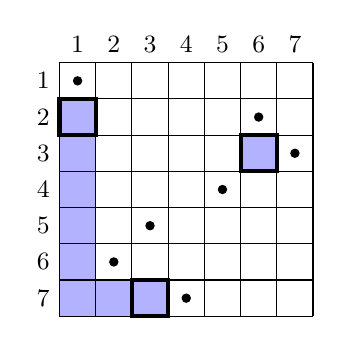
\begin{tikzpicture}[scale=0.46,baseline={([yshift=-2.9mm]current bounding box.center)}]
% Rothe diagram boxes (remaining boxes)
\foreach \c/\r in {
    1/2,
    1/3, 6/3,
    1/4,
    1/5,
    1/6,
    1/7, 2/7, 3/7
}{
    \fill[blue!30] (\c-1,7-\r) rectangle (\c,8-\r);
}
% Draw the 7x7 grid
\draw[step=1,black,thin] (0,0) grid (7,7);
% Permutation matrix pivots: (column i, row w(i))
\foreach \c/\r in {
    1/1,
    2/6,
    3/5,
    4/7,
    5/4,
    6/2,
    7/3
}{
    \fill[black] (\c-0.5,7.5-\r) circle (0.13);
}
% Column labels
\foreach \i in {1,...,7}{
    \node[above] at (\i-0.5,7) {\small \i};
}
% Row labels
\foreach \i in {1,...,7}{
    \node[left] at (0,7.5-\i) {\small \i};
}
\foreach \c/\r in {1/2, 3/7, 6/3} {\draw[black, line width=1.5pt] (\c-1,7-\r) rectangle (\c,8-\r);}
\end{tikzpicture}
\]
Thus, $X_w$ is defined by the rank conditions $\dim_\bC(V_1\cap E_1)\geq 1$, $\dim_\bC(V_3\cap E_6)\geq 3$, and $\dim_\bC(V_6\cap E_2)\geq 2$. Equivalently, $V_1 = E_1$, $V_3 \subset E_6$, and $E_2\subset V_6$.
\end{example}

We now move to defining the cohomology ring of $\fl_n.$ Let $S = \bK[x_1,\ldots,x_n],$ let $e_1,\ldots,e_n$ denote the elementary symmetric polynomials in $x_1,\ldots,x_n$ variables, and let $I_n = (e_1,\ldots,e_n)$ denote the ideal they generate. The quotient $R_n:=S/I_n$ is the \emph{coinvariant algebra} of $\sn.$

\begin{theorem}[\cite{Borel1953}]
\label{thm: Borel - flag variety isomorphism}
    There is an isomorphism of graded rings $H^*(\fl_n,\bK)\cong R_n,$ under which $x_i$ has cohomological degree $2.$ In particular, the odd cohomology of $\fl_n$ vanishes.
\end{theorem}

Concretely, let $0 = \mathcal{S}_0\subset\mathcal{S}_1\subset\cdots\subset\sn = \mathcal{O}^{\oplus n}$ denote the tautological flag of subbundles of $\fl_n,$ and let $L_i = \mathcal{S}_i/\mathcal{S}_{i-1}$ be the associated line bundles. Under the isomorphism of \Cref{thm: Borel - flag variety isomorphism}, the variable $x_i = -c_1(L_i),$ and the relations $e_i = \cdots = e_n = 0$ correspond to the triviality of the total Chern class of $\bigoplus_i L_i\cong\mathcal{O}^{\oplus n}.$

Since $e_1,\dots, e_n$ are algebraically independent, they form a regular sequence. Taking the Koszul resolution of $R_n$ over $S$ and computing the Hilbert series, we obtain
\[
\hilb(R_n;t) = \prod_{i=1}^n(1-t^i)\cdot(1-t)^{-n} = \prod_{i=1}^n(1+t+\cdots+t^{i-1}) = [n]_t!,
\]
where $[k]_t := 1+t+\cdots + t^{k-1}$ and $[k]_t! := [1]_t\cdots [k]_t.$ 
In particular, $\dim_\bK R_n = n!,$ the top nonvanishing graded piece of $R_n$ sits in degree $\binom{n}{2}$ and is one dimensional. $R_n$ also satisfies Poincar{\'e} duality between graded pieces in degrees $k$ and $\binom{n}{2}-k.$ Comparing the above with the standard identity $\sum_{w\in\sn}t^{\ell(w)}=[n]_t!$ verifies that the graded dimensions of $R_n$ are the number of permutations of each length. Furthermore, $H^*(\fl_n;\bK)$ has a basis indexed by $\sn$ and given by the classes of the Schubert varieties $X_w.$ (We make this explicit in the next section.) 

%---------------------------------------------------------------
\subsection{Schubert polynomials and the cohomology ideals \texorpdfstring{$J_w$}{Jw} of Schubert varieties}
\label{subsec: Schubert stuff}
%---------------------------------------------------------------
The coinvariant algebra $R_n = S/(e_1,\ldots,e_n),$ where $e_i$ is the $i$th elementary symmetric function, has a basis given by the Schubert polynomials $\fraks_w$ (\Cref{def: schubert polynomials}), which are in bijection with the permutations of $\sn.$ 
This basis has a direct correspondence to the geometry of the flag variety \cite{Borel1953}, as we recall below. 

We begin this section by introducing the divided difference operator, which are used to define the Schubert polynomials. We then define the ideal $J_w$ and record some cases in which a convenient generating set of $J_w$ is known. In particular, we highlight work of Gasharov-Reiner \cite{GasharovReiner} which studies the case of $X_w$ being defined by inclusion conditions. In that case, $J_w$ is generated by elementary symmetric polynomials in initial and final blocks of the variables. 


\begin{definition}
\label{def:div-diff}
For \(1\leq i<n\), the divided-difference operator is
\[
\partial_i(f(x))=\frac{f(x)-s_i(f(x))}{x_i-x_{i+1}},
\]
where $s_i(f(x))$ is the result of swapping variables $x_i$ and $x_{i+1}$ in $f(x)$. 
If $v = s_{i_1}\cdots s_{i_p}$ is a reduced expression for a permutation $v$, define $\partial_v=\partial_{i_1}\cdots\partial_{i_p}$.
This definition is independent of the choice of reduced word \cite[Chapter II, Equation (2.5)]{Macdonald}.  
\end{definition}

Since $I_n$ is generated by symmetric polynomials and each $\partial_i$ is linear over the ring of symmetric polynomials in $x_i,\ldots,x_n$, then $\partial_i(I_n)\subseteq I_n.$ 
Each $\partial_i$ therefore descends to a well-defined operator on $R_n,$ and hence so does every $\partial_v.$
The divided difference operators act on squarefree monomials in a predictable and simple way, which we record here for later calculations.

\begin{remark}
\label{rem:sqfr-mon-div-diff}    
On a squarefree monomial,
\begin{equation}
\label{eq:squarefree-dd}
 \partial_i(x_F) = 
 \begin{cases}
 x_{F\setminus\{i\}},&i\in F,\ i+1\notin F,\\
 -x_{F\setminus\{i+1\}},&i\notin F,\ i+1\in F,\\
 0,&\text{otherwise}.
 \end{cases}
\end{equation}
\end{remark}

The Schubert polynomials are defined by applying divided difference operators to the \emph{top degree staircase monomial}.

\begin{definition}[\cite{lascoux-schutzenberger}]
\label{def: schubert polynomials}
    Let $w_0 = n(n-1)\cdots 1$ be the longest element of $\sn$ and define
    \[
    \fraks_{w_0} := x_1^{n-1}x_2^{n-2}\cdots x_{n-1}.
    \]
    The \emph{Schubert polynomial} of a permutation $w\in\sn$ is
    \[
    \quad \fraks_w:=\partial_{w^{-1}w_0}(\fraks_{w_0}).
    \]
    Since $\ell(w^{-1}w_0) = \binom{n}{2} - \ell(w)$ and $\partial_v$ lowers degree by $\ell(v),$ the polynomial $\fraks_w$ is homogeneous of degree $\ell(w).$
\end{definition}

The following records the two properties of this construction that we use, namely that it produces a basis and that it is compatible with grading.

\begin{proposition}[\cite{Macdonald,lascoux-schutzenberger}]
\label{prop: schuberts form a basis for Rn}
    The set $\{\fraks_w:w\in\fraks_n\}$ is a $\bK$-basis for $R_n.$ In particular, $\dim_\bK(R_n)_k$ is the number of permutations in $\fraks_n$ of length $k.$
\end{proposition}

We will also need the following relative divided-difference operators in the proof of our main theorem.
\begin{definition}\cite{Macdonald}
\label{def:relative-diff-oper} 
The relative/skew divided-difference operators \(\partial_{u/v}:S\to S\) are defined as the unique linear operators which obey the generalized Leibniz rule 
\begin{equation}
\label{eq:generalized-leibniz}
 \partial_u(fg) = \sum_{v\leq u}
 v\!\left(\partial_{u/v}f\right)\partial_vg.
\end{equation}
\end{definition}

\begin{remark}
    Note that the operators $\partial_u$ and $\partial_{u/v}$ lower the degree by $\ell(u)$ and $\ell(u)-\ell(v),$ respectively \cite[Ch.~II,~Eq.~2.17]{Macdonald}.
\end{remark}

\begin{definition}
\label{def:linear-functionals}
As the Schubert polynomials form a basis for $R_n$ as a $\mathbb{K}$-vector space, there are functionals $\lambda_v:R_n \to \mathbb{K}$ such that  $\lambda_v(\mathfrak{S}_u) = \delta_{u,v}$, where $\delta_{u,v}$ is the Kronecker delta function.
\end{definition}

\begin{remark}
\label{rem:lin-func-length}
If \(f\in(R_n)_{\ell(v)}\) where $\ell(v)$ is the minimum length of $v$ as a reduced word as a product of simple transpositions, then by \cite[Ch.~IV,~Eq.~4.2]{Macdonald} we have
\begin{equation}
\label{eq:coefficient-dd}
 \lambda_v(f)=\partial_v(f).
\end{equation}
\end{remark}

A \textbf{Schubert variety} $X_w$ is a subvariety of $\fl_n$ cut out by certain rank conditions of the form $\dim(V_a\cap E_b)\geq c$ on the moving flag $V_\bullet$ \cite[Ch.~1]{Handbook}. 
Each Schubert polynomial $\fraks_w\in R_n$ is a representative of the cohomology class $[X_w]$ of the Schubert variety corresponding to $w$.

The Schubert varieties $X_w$ are the cell closures of a cell decomposition of $\fl_n$ by Schubert cells. Since each Schubert variety is the union of the Schubert cells that are contained in it, the map on cohomology $\iota^*:R_n\cong H^*(\fl_n;\bK)\to H^*(X_w;\bK)$ induced by the inclusion $\iota:X_w\subseteq \fl_n$ is surjective. Define $J_w\coloneqq \ker(\iota^*)$. By general facts about cohomology, see for example~\cite{ReinerWooYong}, 
\begin{equation}\label{eq: Jw}
J_w = \mathrm{span}_\bK\{\fraks_v:v\in\sn,v\not\leq w\}\subseteq R_n.
\end{equation}

We can also extend the concept to intersections of ideals.
\begin{lemma}
\label{lem: surjective map on homology from flag var to union}
    Let $\calW\subseteq\sn$ be a Bruhat antichain, let $X_\calW = \bigcup_{w\in\calW}X_w,$ and let $J_\calW$ be the kernel of the restriction map $\iota^*:R_n\cong H^*(\fl_n;\bK) \to H^*(X_\calW;\bK).$ Then $\iota^*$ is surjective and 
    \[
    J_\calW = \bigcap_{w\in\calW} J_w = \mathsf{span}_{\bK}\{\fraks_v:v\not\leq w \text{ for every }w\in\calW\}+I_n.
    \]
\end{lemma}
\begin{proof}
    The union of $X_\calW$ is the union of Schubert cells $C_v,$ for $v\leq w$ and $w\in \calW$, and every cell has even real dimension. Therefore, $H_*(X_\calW;\bK)$ has a basis $\{[X_v] : v\leq w,\, w\in \calW\}$ and $H^*(X_\calW;\bK)$ is its dual under the cap product pairing. Since $X_\calW$ is a closed union of cells, the map
    \[
    H^*(\fl_n;\bK)\to H^*(X_\calW;\bK)
    \]
    sends each class $[X_v]$ in $H^*(\fl_n;\bK)$ to either $[X_v]$ in $H^*(X_\calW;\bK)$ if $X_v\subseteq X_{\calW}$ or to $0$ otherwise. Thus, the map is surjective with kernel spanned by the $[X_v]=\fraks_v$ for $v\not\leq w$ for all $w\in \calW$.
\end{proof}


\begin{comment}
Alternate proof.
\begin{proof}
    The union of $X_\calW$ is the union of Schubert cells $C_v,$ for $v\leq w$ and $w\in \calW$. 
    Every cell has even real dimension. 
    So $H_*(X_\calW;\bK)$ has a basis $\{[X_v] : v\leq w,\, w\in \calW\}$ and $H^*(X_\calW;\bK)$ is its dual under the cap product pairing. The same statement holds for $\fl_n$ and for each $X_w.$ 
    The inclusion $X_\calW\subseteq\fl_n$ is therefore injective on homology, so $i^*$ is surjective. 

    Each $[X_v]$ is the image of a class in $H_*(X_w;\bK)$ for some $w\in\calW$ with $v\leq w.$ 
    Thus,
    \[
    H^*(X_\calW;\bK)\longrightarrow\bigoplus_{w\in\calW} H^*(X_w;\bK)
    \]
    is injective.
    It follows that a class in $H^*(\fl_n;\bK)$ restricts to zero on $X_\calW$ if and only if it restricts to zero on $X_w$ for every $w\in\calW,$ that is, $J_\calW = \bigcap_{w\in\calW}J_w.$

    The last equality follows from \Cref{eq: Jw}, since each $J_w$ is spanned by a subset of the Schubert basis of $R_n.$
\end{proof}
\end{comment}

Recall that the essential set of $w$ identifies a minimal collection of incidence conditions defining $X_w.$ We are concerned with certain permutations for which these conditions take on a rather simple form.

\begin{definition}[\cite{GasharovReiner}]
    A Schubert variety $X_w$ is \emph{defined by inclusions} if it is cut out by conditions of the form $E_a\subseteq V_b$ and $V_b\subseteq E_a$ alone.
\end{definition}

Remarkably, this class of Schubert varieties is detected by pattern avoidance. 

\begin{theorem}[\cite{GasharovReiner}]
    The Schubert variety $X_w$ is defined by inclusions if and only if $w$ avoids the patterns $4231,35142,42513,$ and $351624.$
\end{theorem}

\begin{proposition}[\cite{ReinerWooYong}]\label{prop:e-relations}
    Suppose $X_w$ is defined by inclusions. Then $J_w$ is generated by
    \[
    \{e_m(x_1,\ldots,x_r): m = r-s+1,\ldots,r\}\quad\text{for each condition }E_s\subseteq F_r,
    \]
    \[
    \{e_m(x_{r+1},\ldots,x_n): m = s-r+1,\ldots,n-r\}\quad\text{for each condition }F_r\subseteq E_s.
    \]
\end{proposition}

Finally, we isolate the part of an ideal generated by its squarefree monomials, which is of particular importance for us. We note that the following definitions are non-standard.
\begin{definition}
\label{def:sqfr-mon-subideal}
For a homogeneous ideal \(I\subseteq R_n\), define the following ideal in $R_n$,
\[ \mathrm{SqfMon}(I)=\left( x_F:F\subseteq[n],\ x_F\in I\right). \]
\end{definition}

\begin{remark}
\label{rem:sqfr-mon-subideal}
In other words, \(\mathrm{SqfMon}(I)\) is the ideal generated by all squarefree monomials  in \(I\), so
\[ I\text{ is generated by squarefree monomials}\quad\Longleftrightarrow\quad \mathrm{SqfMon}(I)=I.
\]
\end{remark}

\begin{definition} \label{def:forbidden-ascents} 
Fix \(w\in S_n\) with \(w\neq\mathrm{id}\), where \(w(k)=k\) for \(k\notin[i,j]\), $w(i)\neq i$, and $w(j)\neq j$. 
Set 
\[ A(w):=\mathrm{Des}_L(w)^c\cap[i+1,j-2]\]
where $\mathrm{Des}_L(w)$ is the set of left descents of $w$, i.e, 
\[\mathrm{Des}_L(w) := \left\{q\in[n-1]\;:\;w^{-1}(q+1)<w^{-1}(q)\right\}.\]
\end{definition}

\begin{remark}
\label{rem:forbidden-ascents}
For $q\in[i+1,j-2]$,  \(q\in A(w)\) exactly when\footnote{as this is exactly when $\ell(s_q(w)) = \ell(w)+1$} \(w< s_qw\), and $w\in S_n(\mathcal{P})$ exactly when $A(w) = \varnothing$. (See \Cref{lem:AvoidEquivDecrease}.)
\end{remark}
